\chapter{FPGA Stuff, title this better.}

\note{
  Need to clean this up for thesis...
  Need to put refs from here into the .bib
}

\section{Theory}
To take full advantage of the unique characteristics of highly irregular SpMV operations, this chapter a new streaming multi-format structure. Where single-format matrices may succeed in general or uniform cases, there are others where the sparsity is not uniform. In these cases it may be beneficial to store parts of the larger matrix in the most efficient format. As well, because each value in a matrix for matrix-vector multiplication is read from only once, a streaming data structure may be particularly suited to the task. Furthermore, because of the heterogeneous logic involved in the different algorithms tailored to the different formats, current GPU hardware accelerators may not be sufficient, should any type of parallelism be pursued. Therefore, to address this unique challenge, this chapter proposes implementing this structure on FPGA. In summary, this chapter will discuss a multi-format matrix block stream, in which block sizes may be of arbitrary granularity and of arbitrary format to best exploit the data layout on a matrix by matrix basis.

\section{Mechanism}
\subsection{Implementation}
\begin{figure}[htbp]
    \centering
    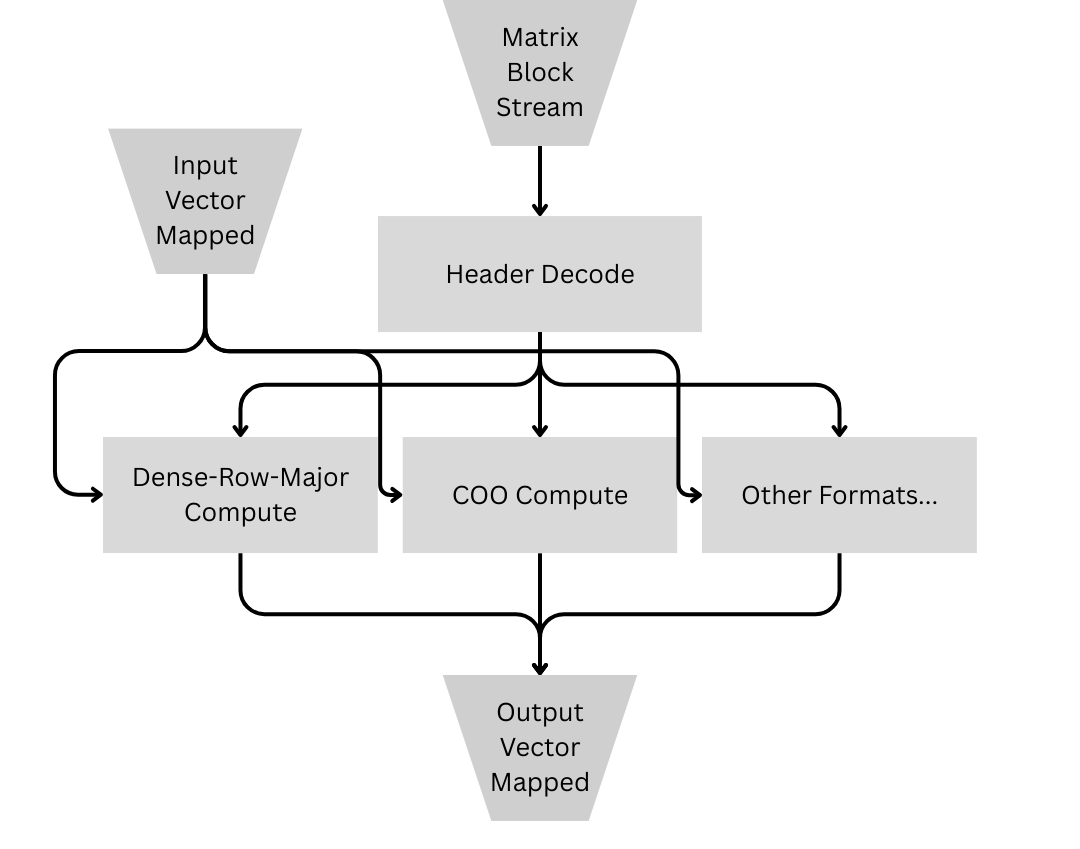
\includegraphics[width=0.9\linewidth]{figures/current_impl.png}
    \caption{Current Sequential Implementation}
    \label{fig:curr_impl}
\end{figure}
In this initial exploratory implementation, Figure~\ref{fig:curr_impl}, only two simple submatrix format options were chosen: Sparse coordinate (COO) and dense row-major / C-style. These were chosen for the simplicity of streaming. As well \cite{overcoming-irreg} found it to be quite resistant to very irregular matrices, meaning a smaller variance. In matrix-vector multiplication, each element of the matrix must only be visited/read from once, making a stream a satisfactory data structure for storing and retrieving matrix elements as they are needed. Vitis also provides the hls::stream library for just this purpose. By default, this wraps around a FIFO port when placed on the top interface, so out of order accesses are not allowed \cite{xilinx_guide}. This constraint is not an issue for the two formats chosen. The test bench takes matrices already in COO format sorted by row, then column and divides them into blocks. Each block is tested for a simple threshold of sparsity:
\begin{equation}
\text{Format} =
\begin{cases}
\text{Dense Row-Major}, & \text{if } 8mn \leq 24nnz, \\
\text{COO}, & \text{otherwise}.
\end{cases}
\end{equation}
Here, \(m\) and \(n\) denote the number of rows and columns in the block, respectively, and \({nnz}\) is the number of non-zero elements in the block. The constants 8 and 24 represent the number of bytes required to store one element in dense and COO formats, respectively. This heuristic favors dense format when its storage cost is less than or equal to that of COO. Future work may explore more sophisticated format-selection rules.

After format-selection, a header is constructed for the data:
\begin{lstlisting}[float, language=C, caption={Block header structure for mixed-format streaming.}, label={lst:block-header}]
struct Mix_Matrix_Header
{
    Matrix_Format  format;  // Enum: NONE = 0, DENSE = 1, COO = 2
    uint64_t       vec_in_offset;  // Input vector offset
    uint64_t       vec_out_offset; // Output vector offset
    uint64_t       vec_count;  // Number of rows in the tile
    uint64_t       data_size;  // Stream offset to next tile
};
\end{lstlisting}
\begin{figure}[htbp]
    \centering
    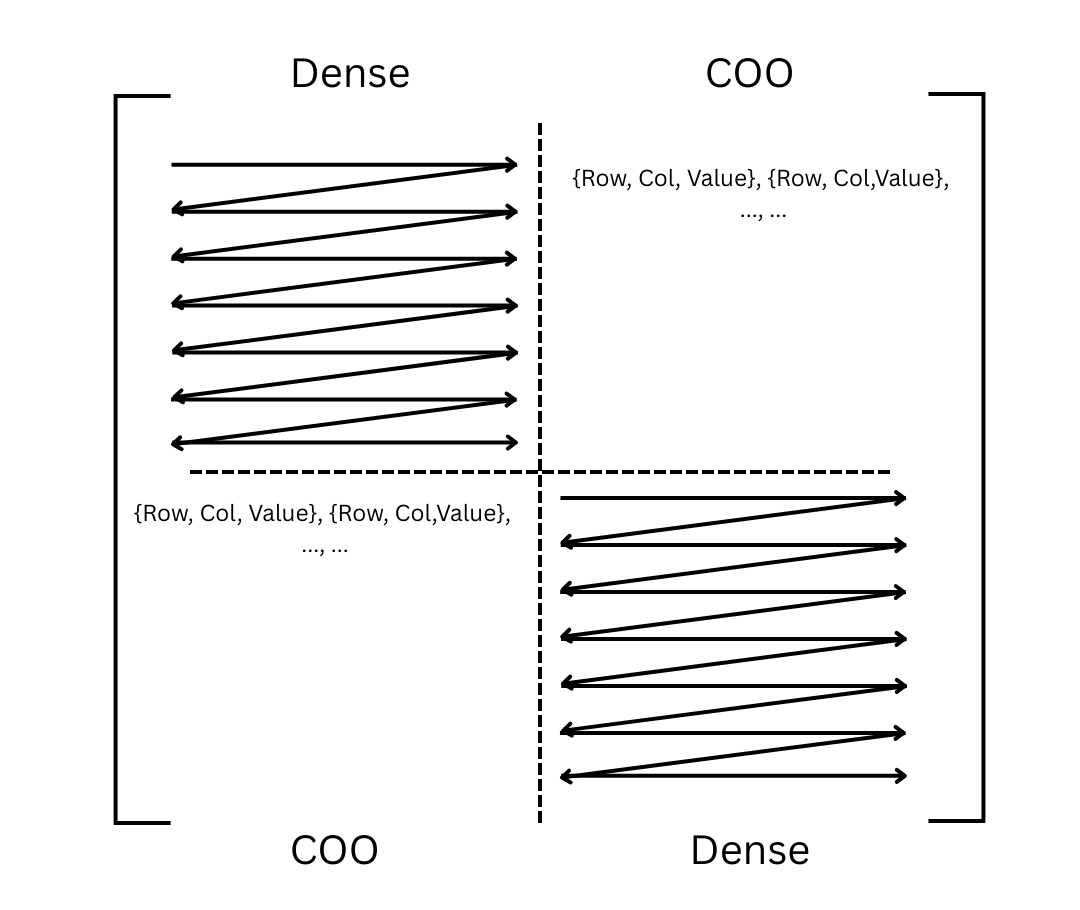
\includegraphics[width=0.9\linewidth]{figures/conceptual.png}
    \caption{Conceptual View of Matrix Stream}
    \label{fig:concept}
\end{figure}
Here, each header contains a bit of information about each following block, most importantly the storage format, and the block offsets into the respective input and output vectors. Matrix data is then written into the stream in the specified format, and in the order the values will be consumed. Values in this implementation are all doubles or 64 bit floats. For the COO format, first the number of non zeroes in the block as a uint64 is streamed, then values are streamed as triples of \({(row, column, value)}\), exactly the order the COO compute function consumes them. And for Dense, first the number of rows and columns in the block are streamed first, again as uint64's, and then values in row major order. Conceptually, it might be thought of as Figure~\ref{fig:concept}.
\begin{table}[htbp]
\centering
\caption{Stream Memory Layout: fixed-size header followed by format-specific data.}
\label{tab:stream-layout}
\begin{tabular}{|c|c|l|}
\hline
\textbf{Bytes} & \textbf{Field}        & \textbf{Description}                \\
\hline
0–39          & Header        & Format ID, offsets, vector count    \\
40–(40+N)     & Dense Payload & \(m \times n \) values\\
...           &                        &                                     \\
X–(X+39)      & Next Header   & Same format as first header         \\
...           & COO Payload   & \(nnz \times (row, col, val)\) triples \\
Y–(Y+39)      & NONE Header   & Signifies the end of the stream   \\
\hline
\end{tabular}
\end{table}

In reality the stream memory layout is demonstrated by Table~\ref{tab:stream-layout}. This stream is then consumed on FPGA, dispatching to the correct format compute function based on the header, Listing~\ref{lst:processing}.

\begin{lstlisting}[float, language=C, caption={HLS Stream Processing on FPGA}, label={lst:processing}]
void mix_matrix_mul_vector_top(Data_Stream *mix_stream,
                               f64 *vec_in, u64 vec_in_count,
                               f64 *vec_out, u64 vec_out_count)
{
  ...
  do
  {
    head = read_matrix_header(mix_stream);

    switch (head.format)
    {
      case Matrix_Format::NONE: { } break;
      case Matrix_Format::DENSE_ROW_MAJOR:
      {
        dense_row_major_mul_vec(mix_stream, head,
                                vec_in, vec_in_count,
                                vec_out, vec_out_count);
      } break;
      case Matrix_Format::COO:
      {
        coo_mul_vector(mix_stream, head,
                       vec_in, vec_in_count,
                       vec_out, vec_out_count);
      } break;
    }
  }
  while (head.format != Matrix_Format::NONE);
}
\end{lstlisting}

\begin{lstlisting}[float, language=C, caption={HLS Stream COO Block Compute}, label={lst:coo_compute}]
void coo_mul_vector(Data_Stream *mix_stream, Mix_Matrix_Header head,
                    f64 *vec_in, u64 vec_in_count,
                    f64 *vec_out, u64 vec_out_count)
{
  u64 non_zero_count = mix_stream->read();

  COO_LOOP:
  for (usize i = 0; i < non_zero_count; i++) {
    u64 coo_row   = mix_stream->read();
    u64 coo_col   = mix_stream->read();
    f64 coo_value = read_f64_from_stream(mix_stream);

    u64 vec_in_index  = coo_col + head.vec_in_offset;
    u64 vec_out_index = coo_row + head.vec_out_offset;

    f64 current   = vec_out[vec_out_index];
    f64 vector_in = vec_in[vec_in_index];

    vec_out[vec_out_index] = current + (coo_value * vector_in);
  }
}
\end{lstlisting}

One can observe that this could be expanded to any number of potential formats, as long as they were conducive to streaming. The compute function/module for COO is given in Listing~\ref{lst:coo_compute}. In hindsight, choosing COO proved to be a little hazardous in the read-modify-write-cycle. Ensuring correctness required disabling pipelining for the COO\_LOOP, greatly limiting potential throughput. This revealed a major limitation of some formats that have very irregular access like COO for the streaming, pipe-lined architecture of FPGAs. This as an important lesson guiding future work in exploring other formats. For now these are relatively naive implementations, but one could imagine using the given format's fastest implementation for each compute module, combining the most effective implementation with the most effective format for each blocks data layout. However, this first implementation is very sequential, having only one stream and writing potentially to the same rows in the memory mapped output vector. Both the input and output vectors are AXI Master memory mapped, since we are accessing these values multiple times. Nonetheless we can take advantage of Matrix-Vector multiplication's need to access each matrix value only once with the use of a streaming data structure.
The tooling used for this implementation was AMD's Vitis HLS suite \cite{xilinx_guide}, and the board we used for our simulations was the Pynq-7000, specifically the xc7z020clg400-1.

\section{Analysis}
\subsection{Preliminary Results}
I created a simple script to generate sparse matrices in edge list format. For this simple exploratory implementation I focused on 2 cases a small 32x32 matrix for initial testing, and a larger matrix of 2048x2048, for a more rigorous test case. In all cases our simple heuristic for deciding format usage achieved a small data footprint, even including stream header overhead, see Table~\ref{tab:memory-usage}. However, the simplicity of the rule leaves much to be desired, and further work should be done, both in finding a more efficient rule perhaps even machine learning based, as Chen et al. have \cite{hybrid_format}, as well as expanding the available formats. However, the implementation leaves much of the available hardware unused, as seen by Table~\ref{tab:fpga-usage}. Ideally, I would like to achieve a much fuller saturation of the DSP units, as well as at least some usage of the fast BRAM. But, there is potential in the streaming structure \cite{fpga-stream}, one could imagine having a much larger sparse matrix that one does not want to materialize all at once. One could instead only materialize by block, and at that moment also decide the format for streaming. This is especially useful as those blocks can then be dematerialized as they are consumed on FPGA, as stated before matrix-vector multiplication only requires one read for any one value of the matrix.
\begin{table}[htbp]
\centering
\caption{Memory Usage for Matrix Size}
\label{tab:memory-usage}
\begin{tabular}{|c|c|c|}
\hline
\textbf{Matrix Dimension} & \textbf{Memory Footprint (KB)} \\
\hline
32x32     & 0.856 \\
2048x2048     & 9827.224   \\
\hline
\end{tabular}
\end{table}

\begin{table}[htbp]
\centering
\caption{FPGA Synthesis Resource Usage}
\label{tab:fpga-usage}
\begin{tabular}{|c|c|c|c|}
\hline
\textbf{BRAM Usage} & \textbf{DSP Usage} & \textbf{LUT Usage} & \textbf{FF Usage}  \\
\hline
2\% & 6\% & 4\% & 10\%        \\
\hline
\end{tabular}
\end{table}



\subsection{Future Work}
Though there is a working implementation, I believe there is much more potential in this idea. So far, the implementation has not fully utilized the strengths of FPGA as a platform, namely parallelism and BRAM usage. Therefore I propose an improvement to the current design, seen in Figure~\ref{fig:reduc_impl}. This design would include alongside the other decode and compute modules, a final reduction module. In this implementation, each block and compute module would receive a slice of BRAM to act as a personal subset of the output vector. In this way, each block could run completely in parallel once it received its data from the stream. A final reduce step would sum any overlapping subset output vectors and write back into the memory mapped true output vector. By allowing compute to be pipe-lined more effectively with reading from the stream, we would hopefully achieve much better memory and resource saturation. As mentioned before, slightly more regularly accessed sparse formats would aid in pipe-lining inner compute loops. In future, I would also like to explore a multiple stream implementation, allowing multiple blocks to be read in parallel.
\begin{figure}[htbp]
    \centering
    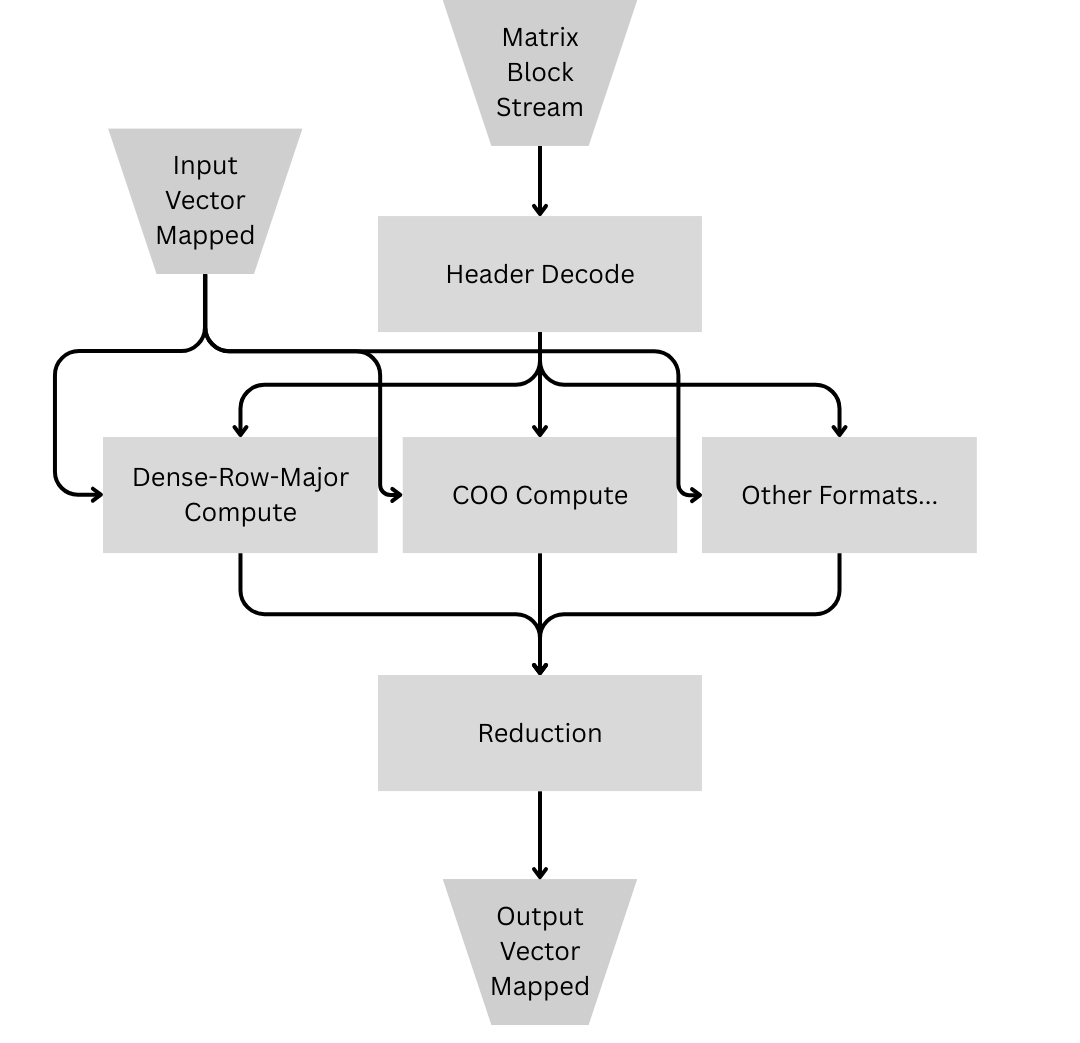
\includegraphics[width=0.9\linewidth]{figures/reduction_impl.png}
    \caption{Future Parallel Implementation}
    \label{fig:reduc_impl}
\end{figure}

\section{Summary}
In conclusion, we have motivated the need for new solutions to very irregular sparse matrices, as well as called attention to previous and older solutions. This chapter proposed a novel streaming structure that might combine the strengths of previous formats, tailoring them to the needed block granularity on an individual matrix basis. In addition, this chapter also describes an implementation of such structure on FPGA to enable future work in parallelizing the heterogeneous computation and unpacking logic of many different formats. Our baseline implementation demonstrated a working computation in which blocks of disparate types were consumed, as well as demonstrated that memory footprint was kept small even with streaming header overhead. Further, this chapter also discussed future work involving usage of BRAM and reduction functional modules for parallelizing computation in hopes of further saturating memory bandwidth.
